\documentclass[12pt, psamsfonts]{amsart}

%-------Packages---------
\usepackage{amssymb,amsfonts}
\usepackage{semantic}
\usepackage{fullpage}
\usepackage{tikz-cd}
\usepackage{todonotes}
\usepackage{physics}
\usepackage[all,arc]{xy}
\usepackage{enumerate}
\usepackage{enumitem}
\usepackage{mathrsfs}
\usepackage{theoremref}
\usepackage{graphicx}
\usepackage[bookmarks]{hyperref}

%--------Theorem Environments--------
%theoremstyle{plain} --- default
\newtheorem{thm}{Theorem}[section]
\newtheorem{cor}[thm]{Corollary}
\newtheorem{prop}[thm]{Proposition}
\newtheorem{lem}[thm]{Lemma}
\newtheorem{conj}[thm]{Conjecture}
\newtheorem{quest}[thm]{Question}

\theoremstyle{definition}
\newtheorem{defn}[thm]{Definition}
\newtheorem{defns}[thm]{Definitions}
\newtheorem{con}[thm]{Construction}
\newtheorem{exmp}[thm]{Example}
\newtheorem{exmps}[thm]{Examples}
\newtheorem{notn}[thm]{Notation}
\newtheorem{notns}[thm]{Notations}
\newtheorem{addm}[thm]{Addendum}
\newtheorem*{exer}{Exercise}

\theoremstyle{remark}
\newtheorem{rem}[thm]{Remark}
\newtheorem{rems}[thm]{Remarks}
\newtheorem{warn}[thm]{Warning}
\newtheorem{sch}[thm]{Scholium}

\DeclareMathOperator{\Hom}{Hom}
\DeclareMathOperator{\Id}{Id}
\DeclareMathOperator{\End}{End}
\DeclareMathOperator{\ord}{ord}
\DeclareMathOperator{\Aut}{Aut}
\DeclareMathOperator{\Gal}{Gal}
\DeclareMathOperator{\CP}{\mathbb{C}P}

\makeatletter
\let\c@equation\c@thm
\makeatother
\numberwithin{equation}{section}

\bibliographystyle{plain}

\begin{document}

\title{Math 612(Homework 5)}
\author{Hidenori Shinohara}
\maketitle

\begin{exer}{(2.2.7)}
  Let $f(x_1, \cdots, x_n) = (-x_1, x_2, x_3, \cdots, x_n)$.
  Then
  \begin{center}
    \begin{tikzcd}[cells={nodes={minimum height=2em}}]
      \mathbb{R}^n \setminus \{ 0 \} \arrow[r, "f"] \arrow[d, "r"]   & \mathbb{R}^n \setminus \{ 0 \} \arrow[d, "r"] \\
      S^{n - 1} \arrow[r, "\text{reflection}"] & S^{n - 1}
    \end{tikzcd}
  \end{center}
  where $r$ is the obvious deformation retraction.
  By (e) on P.134, the reflection map induces -1 on $H^{n - 1}(S^{n - 1})$.
  By naturality, $f_{\ast}$ is -1.

  Similarly, let $f(x_1, \cdots, x_n) = (cx_1, x_2, x_3, \cdots, x_n)$ with $c > 0$.
  Then
  \begin{center}
    \begin{tikzcd}[cells={nodes={minimum height=2em}}]
      \mathbb{R}^n \setminus \{ 0 \} \arrow[r, "f"] \arrow[d, "r"]   & \mathbb{R}^n \setminus \{ 0 \} \arrow[d, "r"] \\
      S^{n - 1} \arrow[r, "g"] & S^{n - 1}
    \end{tikzcd}
  \end{center}
  where $r$ is the obvious deformation retraction.
  Then $g$ is a function that is homotopy equivalent to the identity map on $S^{n - 1}$.
  By (e) on P.134, $g$ induces the identity map on $H^{n - 1}(S^{n - 1})$.
  By naturality, $f_{\ast}$ is 1.

  Using the exact same argument, $(x_1, \cdots, x_i, \cdots, x_j, \cdots, x_n) \mapsto (x_1, \cdots, x_j, \cdots, x_i, \cdots, x_n)$ induces -1 because a reflection is -1 and $(x_1, \cdots, x_i, \cdots, x_j, \cdots, x_n) \mapsto (x_1, \cdots, x_i, \cdots, x_j + x_i, \cdots, x_n)$ induces 1 because homotopy equivalent maps induce the same map.
  Therefore, we have shown that elementary matrices induce 1 or -1 based on the sign of their determinants.
  Any invertible linear operation can be written as a product of elementary matrices and since $(fg)_{\ast} = f_{\ast}g_{\ast}$ the given invertible linear operation induces 1 or -1 based on the sign of their determinants.
\end{exer}

\begin{exer}{(3.3.1)}
  Let $A, B$ be two copies of $\mathbb{R}_{\geq 0}$.
  Consider the space $X$ obtained from $A \cup B$ and the relation $a \sim b$ whenever $a = b = 0$ or $a = b > 1$.
  Then such a space is clearly second countable and locally homeomorphic to $\mathbb{R}$.
  For each point $x \in X$, $H_1(\mathbb{R}^1, \mathbb{R}^1 - \{ x \}) = H_0(S^0) = \{ [-1], [1] \}$ because $S^0$ consists of two points -1, 1.
  Therefore, for every point $x \in X \setminus \{ 0 \}$, there are exactly two choices of generators, each of which corresponds to a number larger than $x$ or smaller than $x$, which we will refer to ``positive" and ``negative" for convenience.
  Suppose $X$ is orientable.
  \begin{figure}[!htb]
  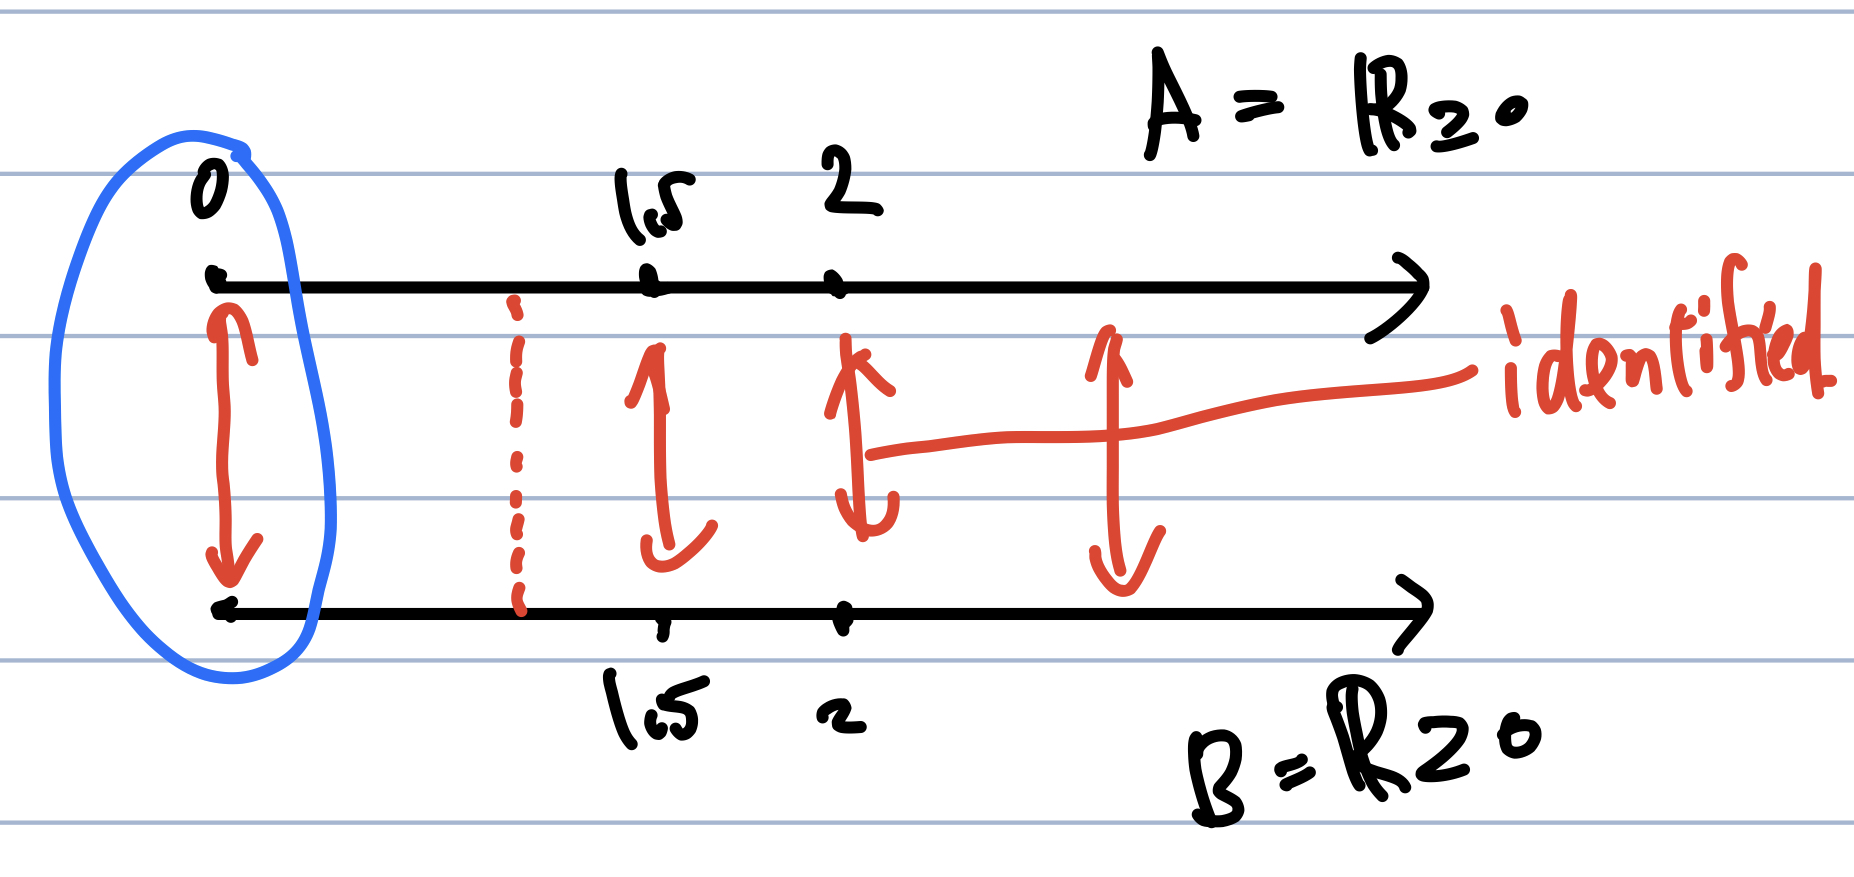
\includegraphics[width=.5\linewidth]{orientability.jpeg}
  \caption{Orientability}
  \label{fig:orientability}
  \end{figure}
  The 0.1 in the blue neighborhood which was originally in $A$ has an orientation that is either positive or negative.
  Without loss of generality, it has the positive orientation.
  This implies that 1 in $A$ has the positive orientation, which in turn implies that all numbers $> 1$ sufficiently close to 1 have the positive orientation.

  Then the 0.1 in the blue neighborhood which was originally in $B$ has an orientation that is negative.
  Therefore, the orientation at 1 which was originally in $A$ has the positive orientation, and 1 which was originally in $B$ has the negative orientation.
  This implies that 1 in $B$ has the positive orientation, which in turn implies that all numbers $> 1$ sufficiently close to 1 have the negative orientation.

  This is a contradiction, so $X$ is not orientable.
\end{exer}

\begin{exer}{(3.3.2)}
  It suffices to consider the case when $M$ is connected because orientations can be chosen for each connected component.
  By Proposition 3.25, $M$ is orientable if and only if an orientable two-sheeted covering space $\tilde{M}$ has two components.
  Each component has exactly one lift of $x$.
  Since the covering map maps some neighborhood of each lift to a neighborhood of $x$ homeomorphically, each component in $\tilde{M}$ is connected after removing the two lifts of $x$.
  Thus $\tilde{M} \setminus \{ \tilde{x}_1, \tilde{x}_2 \}$ is an orientable two-sheeted covering space of $M \setminus \{ x \}$ with two components.
  By Proposition 3.25, $M \setminus \{ x \}$ is orientable.
\end{exer}

\begin{exer}{(3.3.3)}
  Let $\tilde{M}$ be a covering space of an orientable manifold $M$ with a covering map $q$.
  Let $\tilde{x} \in \tilde{M}$ be given.
  Then $H_n(\tilde{M} \mid \tilde{x}) \cong H_n(\tilde{U} \mid \tilde{x})$ where $\tilde{U}$ is a neighborhood of $\tilde{x}$ that is homeomorphically mapped to an open subset $U \subset M$ by $q$.
  Since $M$ is orientable, we have a local orientation $\mu_x \in H_n(U \mid x)$.
  $q$ induces an isomorphism between $H_n(U \mid x)$ and $H_n(\tilde{U} \mid \tilde{x})$.
  Let $\mu_{\tilde{x}} \in H_n(\tilde{M} \mid \tilde{x})$ denote the element corresponding to $\mu_x$ by the isomorphisms.
  This assignment satisfies the local consistency because for each $\tilde{x} \in \tilde{M}$, we pick a small neighborhood $\tilde{B}$ around $\tilde{x}$ that is mapped homeomorphically to a neighborhood $B$ around $x$ by $q$ where $B$ satisfies the local consistency condition around $x$.
\end{exer}

And also the following: Show that there exists a homeomorphism $f: CP^n \to CP^n$ whose induced map on $H^{2n}(CP^n;Z)$ is multiplication by -1 iff n is odd.

\begin{exer}{(Extra)}
  We know that $H^{\ast}(\CP^n; \mathbb{Z}) = \mathbb{Z}[\alpha] / (\alpha^{n + 1})$ where $\abs{\alpha} = 2$.
  Let $f$ be a homeomorphism from $\CP^n$ to itself.
  Suppose $n$ is even.
  Then $f$ induces a homomorphism on $H^n(\CP^n; \mathbb{Z})$ which is generated by $\alpha^{n / 2}$.
  Similarly, $f$ induces a homomorphism on $H^{2n}(\CP^n; \mathbb{Z})$ which is generated by $\alpha^{n}$.
  By naturality, $f^{\ast}(\alpha^n) = (f^{\ast}(\alpha^{n / 2}))^2$.
  Clearly, $(f^{\ast}(\alpha^{n / 2}))^2 \ne -\alpha^n$.
  Suppose $n$ is odd.
\end{exer}


\end{document}


